\documentclass{beamer}
\usepackage[utf8]{inputenc}
\usetheme{Madrid}
\usecolortheme{default}
\usepackage{amsmath,amssymb,amsfonts,amsthm}
\usepackage{txfonts}
\usepackage{tkz-euclide}
\usepackage{listings}
\usepackage{adjustbox}
\usepackage{array}
\usepackage{tabularx}
\usepackage{gvv}
\usepackage{lmodern}
\usepackage{circuitikz}
\usepackage{tikz}
\usepackage{graphicx}

\setbeamertemplate{page number in head/foot}[totalframenumber]

\usepackage{tcolorbox}
\tcbuselibrary{minted,breakable,xparse,skins}



\definecolor{bg}{gray}{0.95}
\DeclareTCBListing{mintedbox}{O{}m!O{}}{%
  breakable=true,
  listing engine=minted,
  listing only,
  minted language=#2,
  minted style=default,
  minted options={%
    linenos,
    gobble=0,
    breaklines=true,
    breakafter=,,
    fontsize=\small,
    numbersep=8pt,
    #1},
  boxsep=0pt,
  left skip=0pt,
  right skip=0pt,
  left=25pt,
  right=0pt,
  top=3pt,
  bottom=3pt,
  arc=5pt,
  leftrule=0pt,
  rightrule=0pt,
  bottomrule=2pt,
  toprule=2pt,
  colback=bg,
  colframe=orange!70,
  enhanced,
  overlay={%
    \begin{tcbclipinterior}
    \fill[orange!20!white] (frame.south west) rectangle ([xshift=20pt]frame.north west);
    \end{tcbclipinterior}},
  #3,
}
\lstset{
    language=C,
    basicstyle=\ttfamily\small,
    keywordstyle=\color{blue},
    stringstyle=\color{orange},
    commentstyle=\color{green!60!black},
    numbers=left,
    numberstyle=\tiny\color{gray},
    breaklines=true,
    showstringspaces=false,
}
%------------------------------------------------------------
%This block of code defines the information to appear in the
%Title page
\title %optional
{4.13.86}

%\subtitle{A short story}

\author % (optional)
{BALU-ai25btech11017}



\begin{document}


\frame{\titlepage}
\begin{frame}{Question}
A plane which is perpendicular to two planes 
\begin{align}
2x - 2y + z = 0 \quad \text{and} \quad x - y + 2z = 4
\end{align}
passes through $(1, -2, 1)$. The distance of the plane from the point $(1, 2, 2)$ is (2006).\\ 
\end{frame}
\begin{frame}{Theoretical Solution}
Let us solve the given equation theoretically and then verify the solution computationally \\
According to the question, \\
Given two planes\\
\begin{align}
\vec{n_1}=\begin{myvec}{2\\-2\\1}\end{myvec}\
\vec{n_2}=\begin{myvec}{1\\-1\\2}\end{myvec}\
\vec{a}=\begin{myvec}{1\\-2\\1}\end{myvec}\
\vec{b}=\begin{myvec}{1\\2\\2}\end{myvec}\
\end{align}
Let $\vec{n}$ be normal vector required plane\\
\begin{align}
\vec{n_1}^T\vec{n}=0\\
\vec{n_2}^T\vec{n}=0\\
\begin{myvec}{\vec{n_1}&&\vec{n_2}}^T\end{myvec}\vec{n}=\begin{myvec}
    {0\\0}
\end{myvec} 
\end{align}
\end{frame}
\begin{frame}{Theoretical Solution}
From solving we
\begin{align}
\vec{n}=\begin{myvec}{1\\1\\0}\end{myvec}
\end{align}
Equation of plane is
\begin{align}
    \vec{n}^T\vec{x}=c\\
    \vec{n}^T\vec{a}=c=-1
\end{align}
distance of point from plane is given by\\
\begin{align}
   k=\frac{\abs{\vec{n}^T\vec{x}-c}}{\|\vec{n}\|}\\
   k=\frac{\abs{\vec{n}^T\vec{b}-c}}{\|\vec{n}\|}=\frac{4}{\sqrt{2}}
\end{align}
\end{frame}
\begin{frame}[fragile]
    \frametitle{C Code}

    \begin{lstlisting}
#include <stdio.h>
#include <math.h>

int main() {
    // Normals of given planes
    double n1[3] = {2, -2, 1};
    double n2[3] = {1, -1, 2};

    // Cross product to get required plane normal
    double a = n1[1]*n2[2] - n1[2]*n2[1];
    double b = n1[2]*n2[0] - n1[0]*n2[2];
    double c = n1[0]*n2[1] - n1[1]*n2[0];

    // Point through which plane passes
    double x0 = 1, y0 = -2, z0 = 1;

    

   

     \end{lstlisting}
\end{frame}
\begin{frame}[fragile]
    \frametitle{C Code }
    \begin{lstlisting}
 // Plane equation: a(x-x0) + b(y-y0) + c(z-z0) = 0
    double d = -(a*x0 + b*y0 + c*z0);

    printf("Equation of required plane: %.1fx + %.1fy + %.1fz + %.1f = 0\n", a, b, c, d);

    // Point from which distance is required
    double x1 = 1, y1 = 2, z1 = 2;

    // Distance formula
    double numerator = fabs(a*x1 + b*y1 + c*z1 + d);
    double denominator = sqrt(a*a + b*b + c*c);
    double distance = numerator / denominator;

    printf("Distance = %.4f\n", distance);

    return 0;
}
    \end{lstlisting}
\end{frame}
\begin{frame}[fragile]
    \frametitle{Python Code}
    \begin{lstlisting}
import numpy as np
import matplotlib.pyplot as plt
from mpl_toolkits.mplot3d import Axes3D

# Plane: x + y + 1 = 0  => normal = (1,1,0)
a, b, c, d = 1, 1, 0, 1  # ax + by + cz + d = 0

# Point
P = np.array([1, 2, 2])

# Distance formula
dist = abs(a*P[0] + b*P[1] + c*P[2] + d) / np.sqrt(a*a + b*b + c*c)
print("Distance =", dist)

# Foot of perpendicular
t = -(a*P[0] + b*P[1] + c*P[2] + d) / (a*a + b*b + c*c)
foot = P + t * np.array([a, b, c])









    \end{lstlisting}
\end{frame}

\begin{frame}[fragile]
    \frametitle{Python Code}
    \begin{lstlisting}
# Grid for plane
x = np.linspace(-5, 5, 20)
y = np.linspace(-5, 5, 20)
X, Y = np.meshgrid(x, y)
Z = np.zeros_like(X)  # since c=0, plane is vertical (no z-dependence)

# Plot
fig = plt.figure(figsize=(8,6))
ax = fig.add_subplot(111, projection='3d')

# Highlighted Plane (solid color + edge lines)
ax.plot_surface(X, Y, Z, color='lightblue', alpha=0.8, edgecolor='k', linewidth=0.5)

# Point
ax.scatter(P[0], P[1], P[2], color='red', s=60, label=f"Point {tuple(P)}")
    \end{lstlisting}
\end{frame}
\begin{frame}[fragile]
    \frametitle{Python Code}
    \begin{lstlisting}
# Foot of perpendicular
ax.scatter(foot[0], foot[1], foot[2], color='green', s=60, label="Foot of perpendicular")

# Distance line
ax.plot([P[0], foot[0]], [P[1], foot[1]], [P[2], foot[2]], 'k--', lw=2, label=f"Distance = {dist:.2f}")

# Labels
ax.set_xlabel("X")
ax.set_ylabel("Y")
ax.set_zlabel("Z")
ax.set_title("Highlighted Plane with Point-to-Plane Distance")

ax.legend()

# Save
plt.savefig("highlighted_plane_distance.png", dpi=300)
plt.show()
     \end{lstlisting}
\end{frame}
\begin{frame}{Plot}
    \centering
    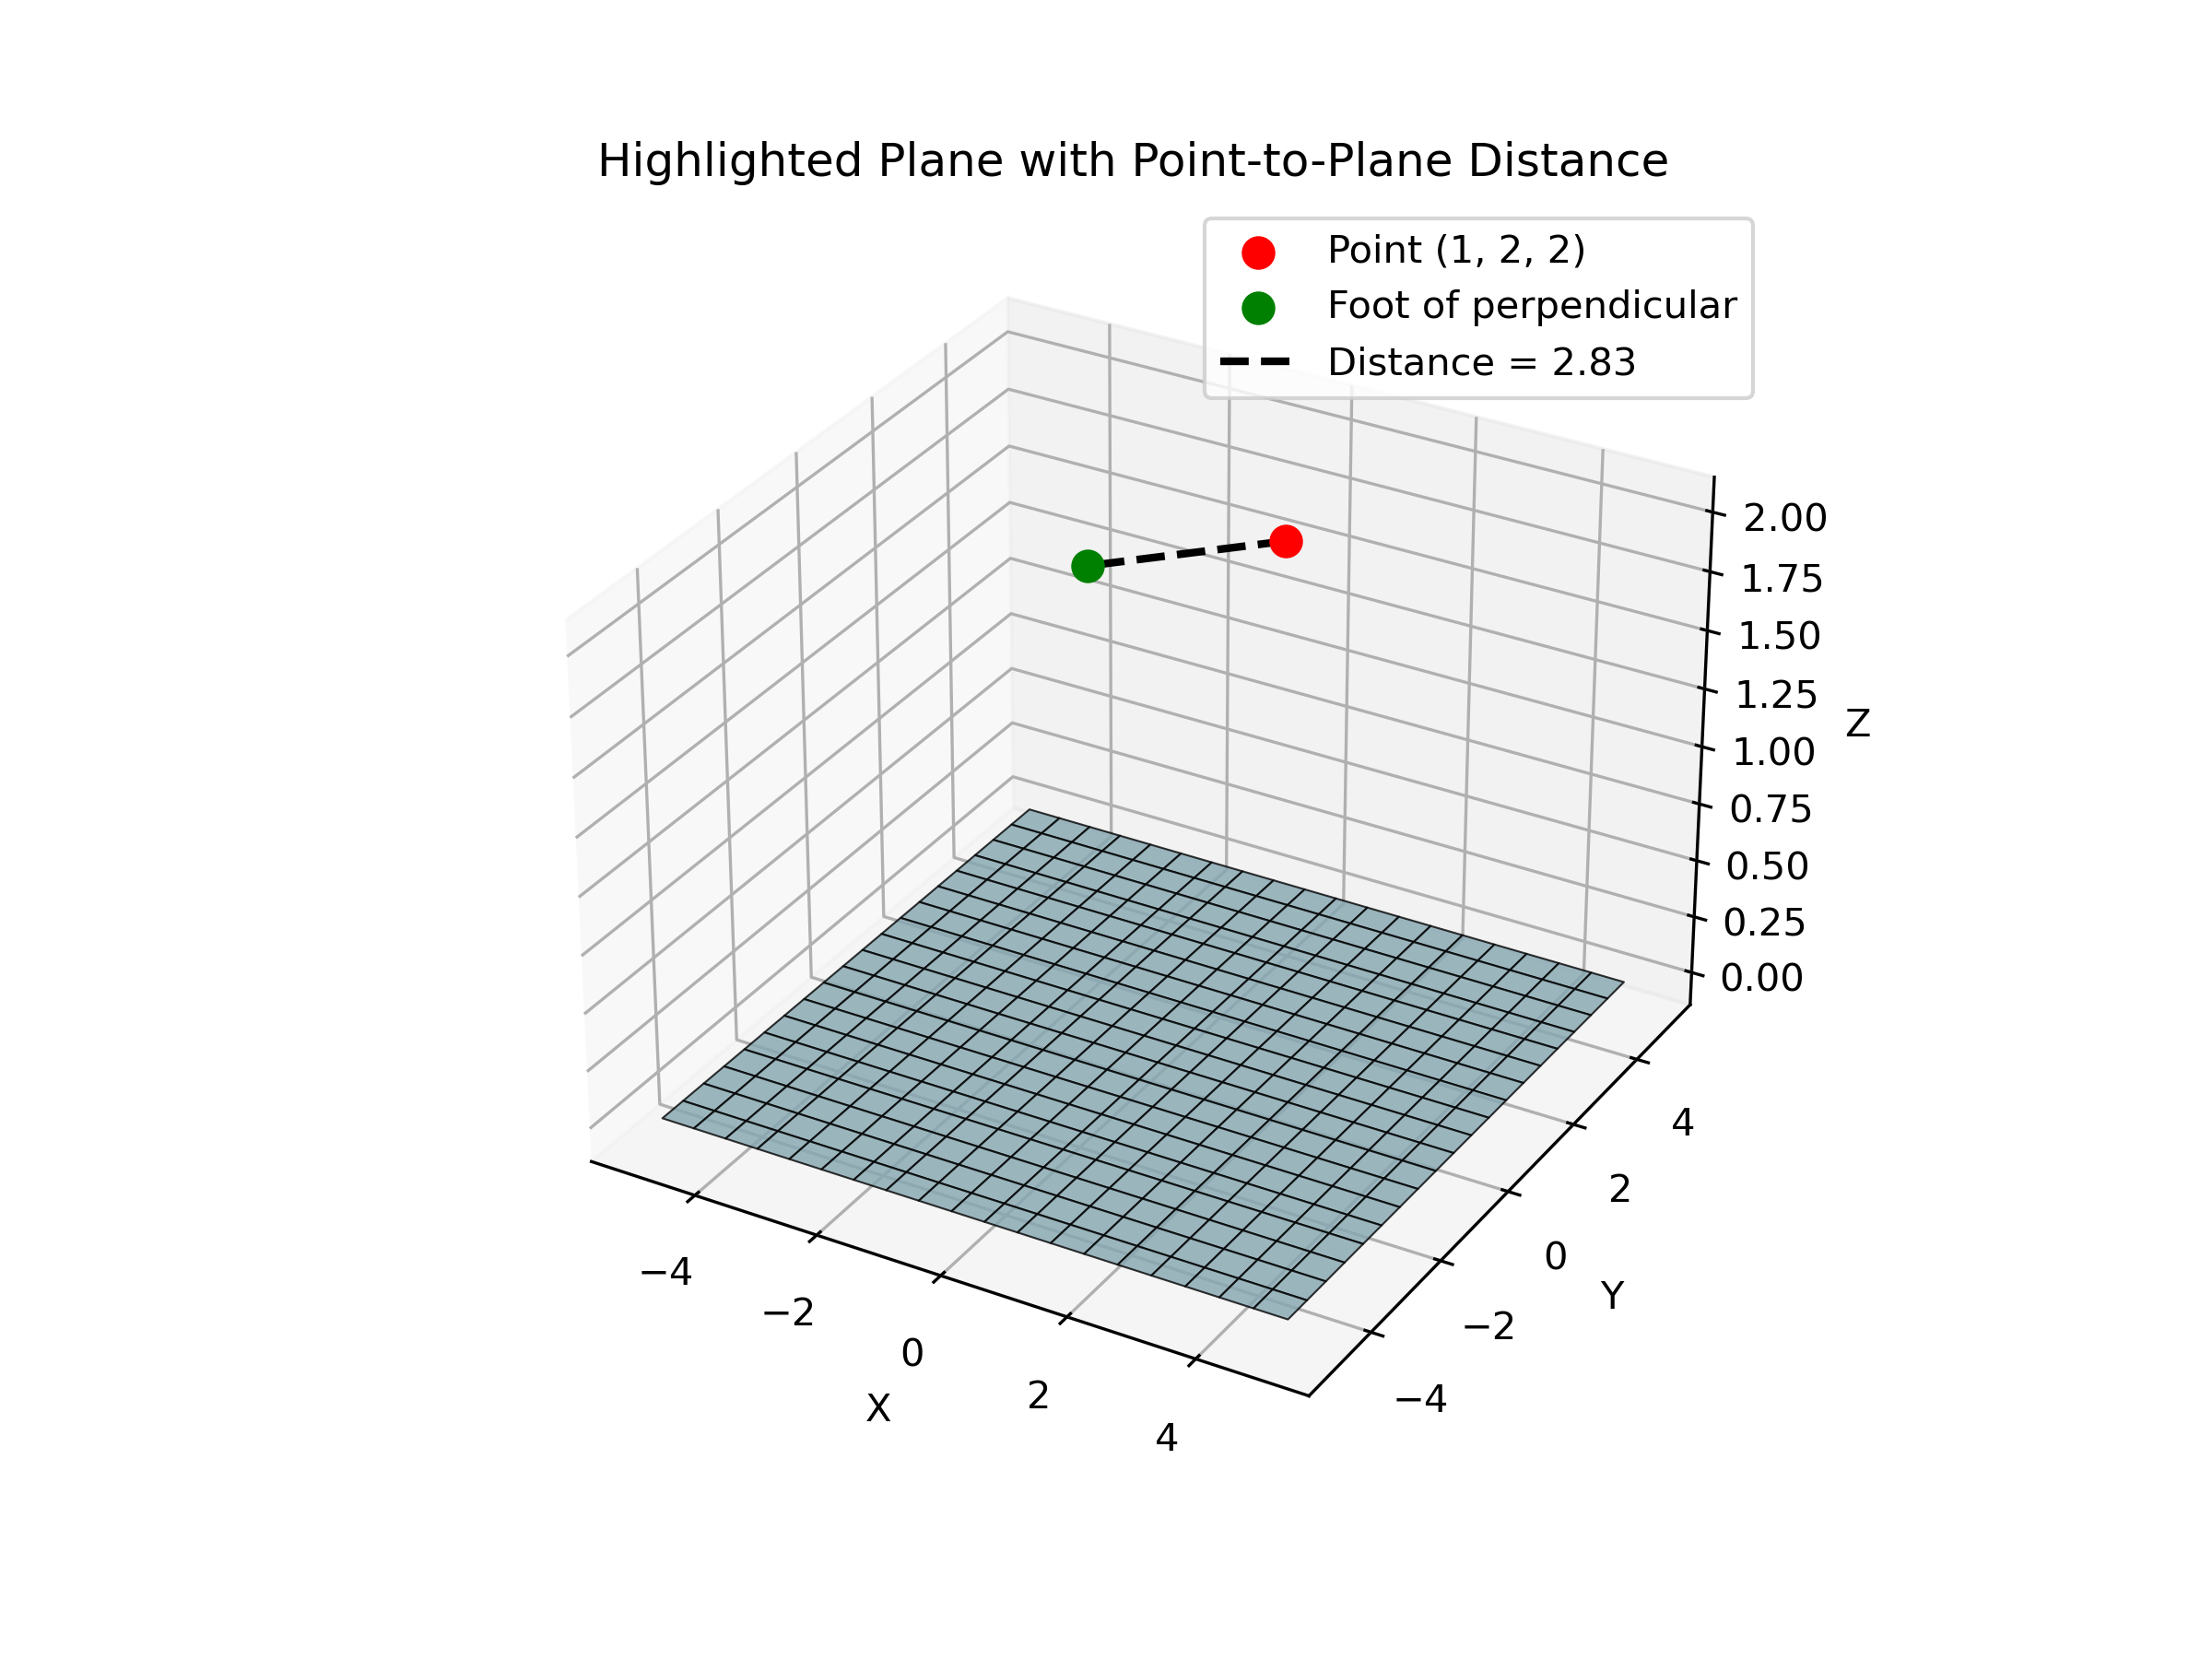
\includegraphics[width=\columnwidth, height=0.8\textheight, keepaspectratio]{figs/highlighted_plane_distance.png}     
\end{frame}




\end{document}